\section{Observation, data analysis and methods}

    \subsection{Data selection}
        %selection criteria of scw: sun activity, elongation and presence of scw
        Given that Venus was never purposely targeted by any of the \textit{INTEGRAL} instruments, the idea was to scan the different science windows (scw) of the
        telescope corresponding to the planet's position in the sky at that moment. Many scw fulfil this condition. Given that planets emit mostly in the softer range
        of the X-ray spectra, only JEM-X data was used\autocite{BhardwajX-raysObjects, Futaana2017SolarAtmosphere}. To ensure the best data quality, other criteria 
        were applied in the data selection. First, scw with increased sun activity were targeted. The sun regained activity following its 11 years cycle in 2021. 
        The April and May 2022 months, with an increase in $\sim$ 79\% and 107\% were appropriate. The elongation of Venus with respect to Earth and the telescope
        were also an important criteria. The elongation represents the Sun-Earth-Venus angle. When the angle is too small, Venus is by construction close to the Sun in the telescope's FoV and hence unobservable(and unobserved by the telescope anyway). \textbf{Fig.} \ref{elongation} illustrates the concept of elongation and \textbf{Fig.} \ref{venus_pos} shows Venus' position during the month of April 2022. The months of April and May 2022 also showed elongation angles close to the maximal value of 47.8°.

    \begin{figure}[H]
        \centering
        
\includegraphics[width = 9cm]{report/Figures/methods/Positional_astronomy.png}
        \caption{Heliocentric diagram of the positional representation of the Earth with respect to inner and outer planets. The greatest elongation is the $\alpha$ angle. It represents the Sun-Earth-Planet angle and is only shown for an outer planet on this diagram.}
        \label{elongation}
    \end{figure}
    
    \begin{figure}[H]
        \centering
        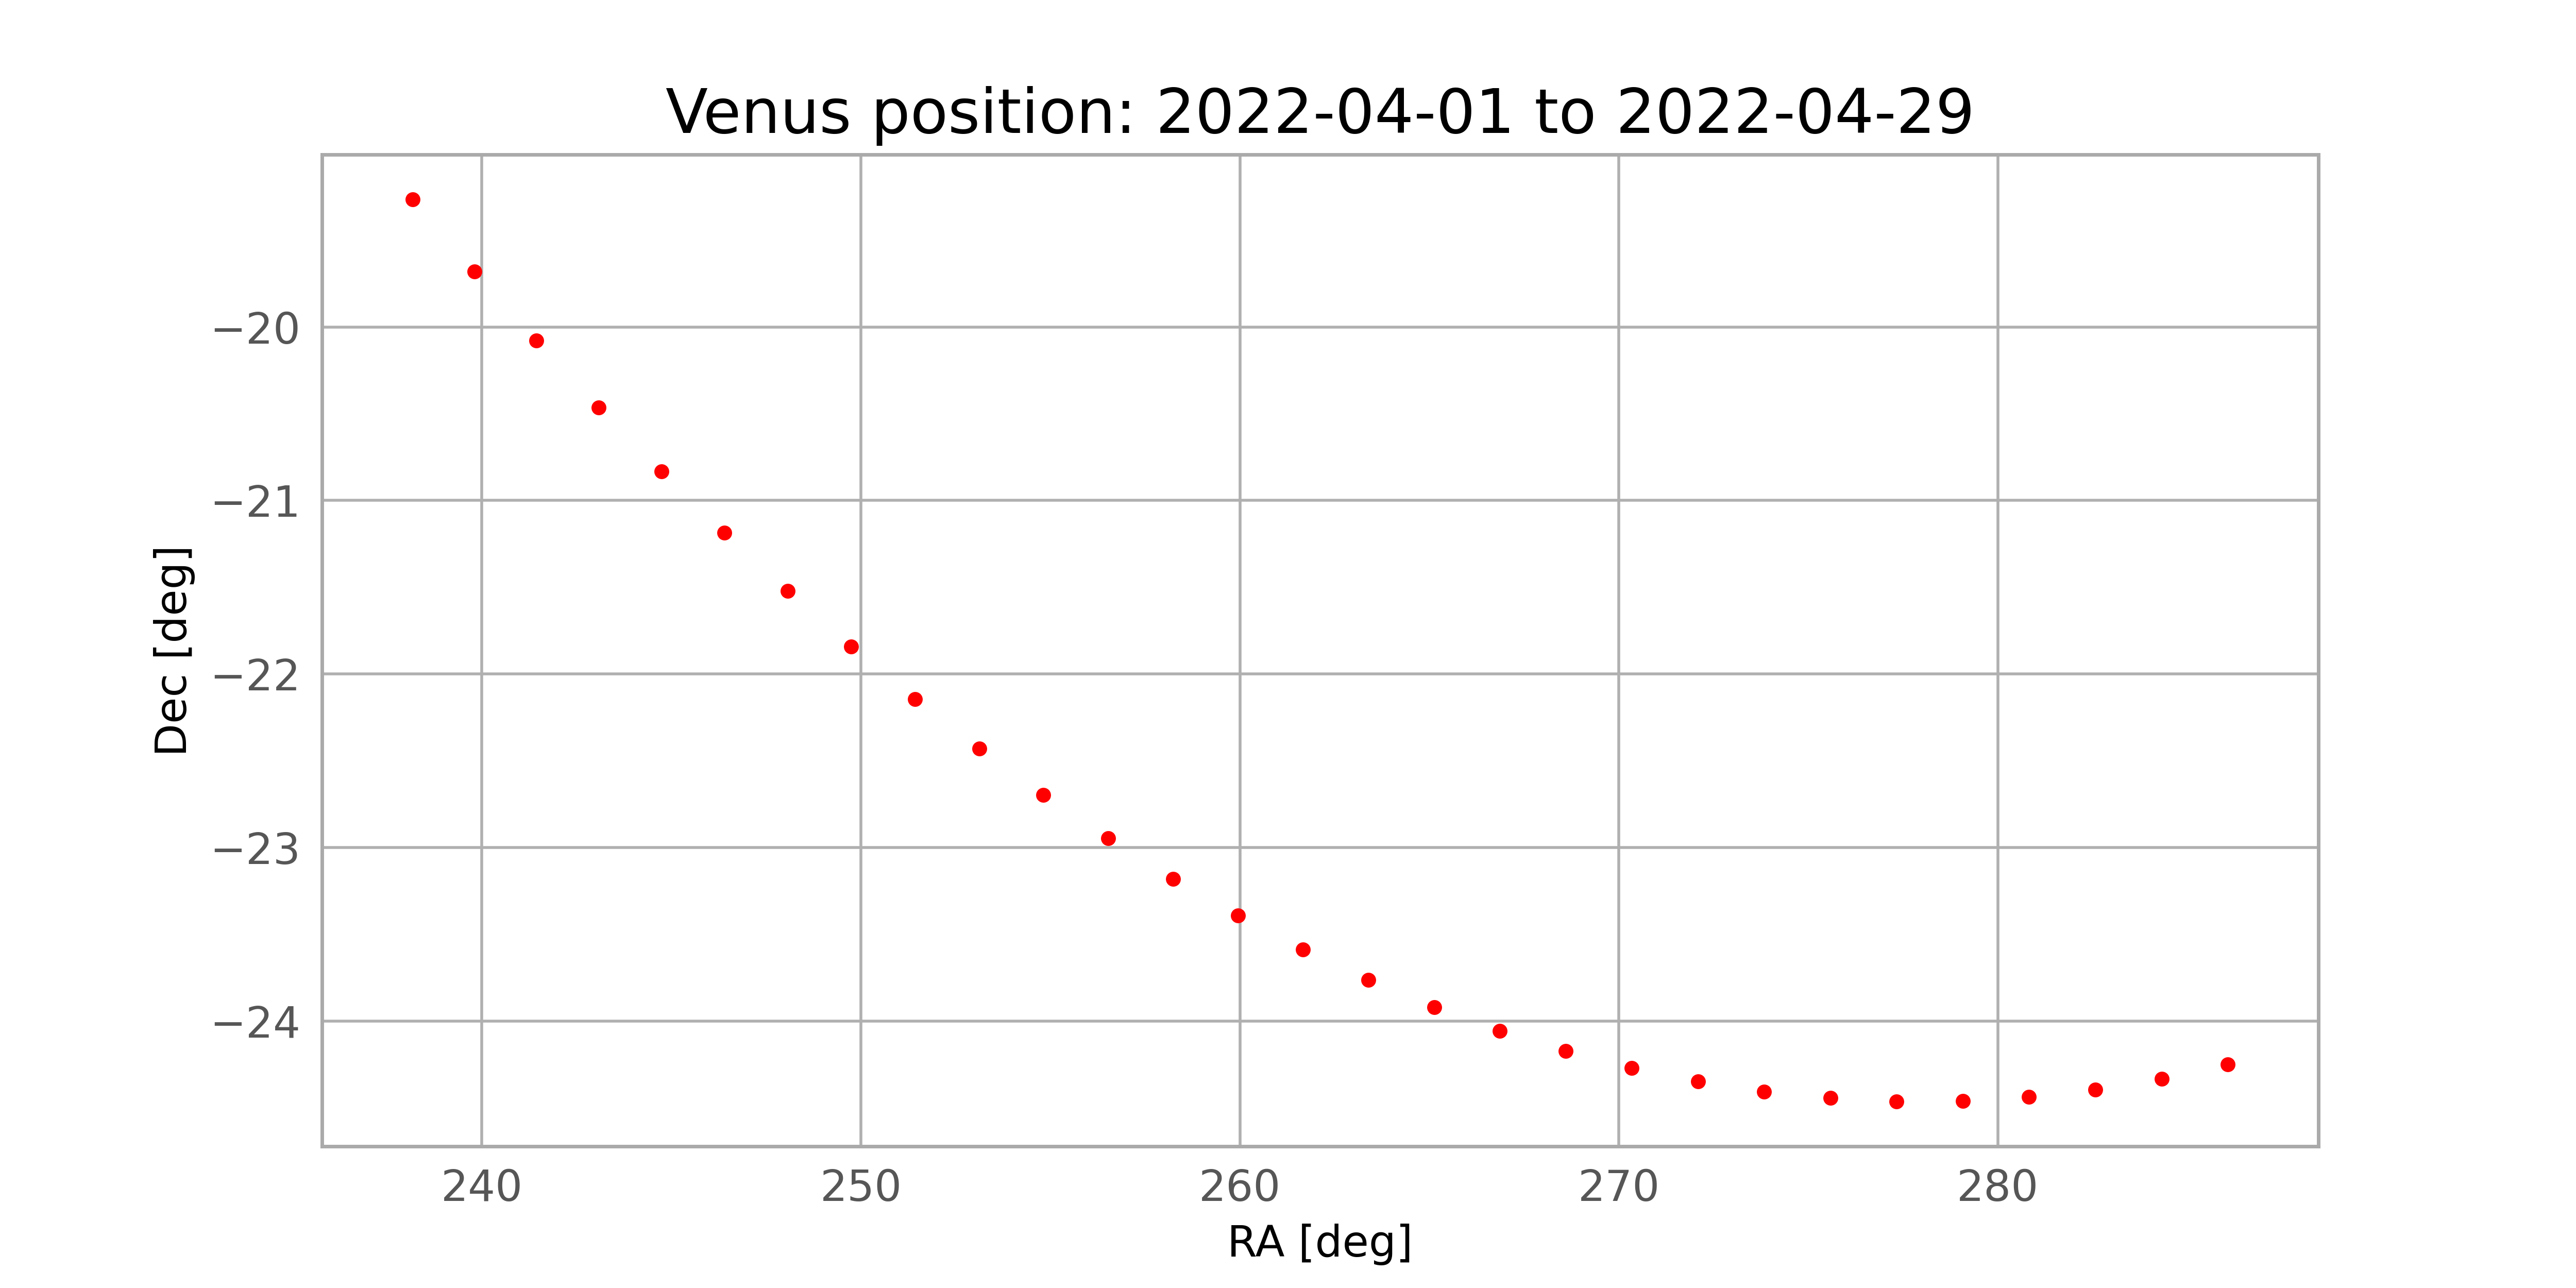
\includegraphics[width = 12cm]{report/Figures/methods/Venus_position.png}
        \caption{Position of Venus every day in the ICRF between the 01.04.2022 and 29.04.2022.}
        \label{venus_pos}
    \end{figure}

        The query was made with the \texttt{ODA-API} given the criteria above and following the parameters listed below:
        \begin{lstlisting}[language = Python,caption = Query parameters template used for both dates.,label = dict]
        par_dict = {
        "E1_keV": "3",
        "E2_keV": "10",
        "detection_threshold": "5",
        "instrument": "jemx",
        "osa_version": "OSA11.2",
        "product": "jemx_image",
        "product_type": "Real",
        "scw_list": scw_list,
        "integral_data_rights": "all-private",#all-private or public
        "token": token
        }
        \end{lstlisting}
        %put some python code, listing with jemx2(radius, energy range etc...) query.
        Quoting \cite{2020ISDCManual}: \textit{In practice, the transmission of the collimator beyond an off-axis angle of 5° is so low that only the very brightest sources can be observed at larger angles}. Therefore, all queries are made with a radius of maximum 5 degrees. The energies probed range from 3 keV to 10 keV. The scws observer identifiers are fed to the API for each date and the data is retrieved in the form of \texttt{fits} files.

        The only scws satisfying these criteria were found in April 2022: four on the 18th, two on the 20th, fourteen on the 22nd and six on the 24th. 
        The data of the 18th and the 20th were eventually not used due to Venus being too excentered in the image. Some scws from the 22nd and 24th were discarded for
        the same reasons.  A summary of all final scws used is shown on \textbf{Tab.} \ref{journal} as well as Venus' characteristics.
        %put characteristics of venus on 22 and 24, put apparent size, pixel size, illumination, elongation, is it approaching or leaving, etc...
        \begin{table}[H]
        \centering
        \begin{tabular}{@{}ccccccc@{}}
        \toprule
        Date                         & scw\textunderscore id       & Time (UTC)          & Elongation [°] & Apparent size [''] & Illumination [\%] & $\Delta$ [AU] \\ \midrule
        \multirow{11}{*}{22.04.2022} & 249400200010 & 04:12:03 - 04:45:23 & 43.88          & 17.89              & 64.30            & 0.93          \\
         & 249400210010 & 04:47:45 - 05:20:55 & 43.88 & 17.89 & 64.31 & 0.93 \\
         & 249400220010 & 05:22:52 - 05:56:13 & 43.88 & 17.89 & 64.32 & 0.93 \\
         & 249400230010 & 05:58:34 - 06:31:43 & 43.87 & 17.88 & 64.33 & 0.93 \\
         & 249400240010 & 06:33:55 - 07:07:14 & 43.87 & 17.88 & 64.34 & 0.93 \\
         & 249400250010 & 07:09:37 - 07:42:45 & 43.87 & 17.88 & 64.34 & 0.93 \\
         & 249400260010 & 07:44:42 - 08:18:03 & 43.85 & 17.87 & 64.35 & 0.93 \\
         & 249400270010 & 08:20:27 - 08:53:35 & 43.85 & 17.87 & 64.36 & 0.93 \\
         & 249400310010 & 10:41:30 - 11:14:50 & 43.85 & 17.87 & 64.37 & 0.93 \\
         & 249400320010 & 11:17:16 - 11:50:21 & 43.84 & 17.87 & 64.37 & 0.94 \\
         & 249400330010 & 11:52:20 - 12:25:41 & 43.84 & 17.86 & 64.38 & 0.94 \\ \midrule
        \multirow{4}{*}{24.04.2022}  & 249500240010 & 19:47:17 - 20:20:27 & 43.50          & 17.52              & 65.33            & 0.95          \\
         & 249500250010 & 20:22:48 - 20:55:58 & 43.49 & 17.51 & 65.34 & 0.95 \\
         & 249500260010 & 20:58:10 - 21:31:29 & 43.49 & 17.51 & 65.35 & 0.95 \\
         & 249500270010 & 21:33:27 - 22:06:47 & 43.48 & 17.50 & 65.36 & 0.95 \\ \midrule 
        \end{tabular}
        \caption{Journal of observations and parameters.
        scw\textunderscore id: science window identifier, $\Delta$: distance from INTEGRAL, Ilumination: fraction of Venus illuminated as seen from observer computed at the beginning of each scw.}
        \label{journal}
        \end{table}

    A noteworthy aspect of targeting an object such as a planet with this telescope is that it moves in the integrated image. Scws last usually between 20min and 1 hour and 
    this is enough for Venus to move in the image of about 1 to 2 pixels.
    
    \textbf{22.04.2022 data}
    
    The April 22 data consists of eleven scws. \textbf{Fig.} \ref{22_map_single} shows the flux map for the first scw of the list shown on \textbf{Tab.} \ref{journal}. The start and end positions of Venus are plotted. A strong source is plotted too using its coordinates retrieved from the \texttt{SIMBAD} server\footnote{\url{https://simbad.unistra.fr/simbad/}} in order to check that Venus' position is plotted correctly since it isn't visually visible on the plot. All the other flux maps are presented in the \textbf{Annex A}. \textbf{Fig.} \ref{22_mosaic} shows a mosaic done using all valid scws from the list with the \texttt{ODA}. All known strong gamma-ray and X-ray sources appearing in each scw are plotted.
    

        \begin{figure}[H]
        \centering
        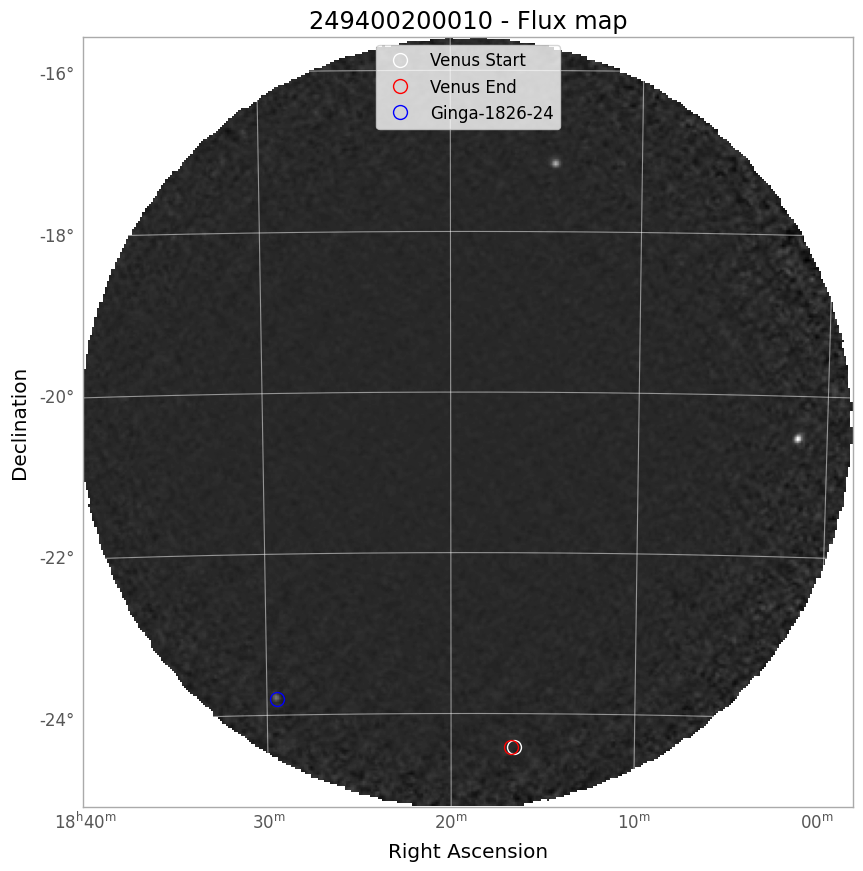
\includegraphics[width = 8cm]{report/Figures/methods/2204/20_map.png}
        \caption{Flux map from the first scw where Venus is present on the 22.04.2022. The start and end positions of Venus are circled in white and red respectively. Another bright source is also plotted to verify the correct localisation approach. Here it is the X-ray binary Ginga 1826-24.}
        \label{22_map_single}
        \end{figure}

        \begin{figure}[H]
        \centering
        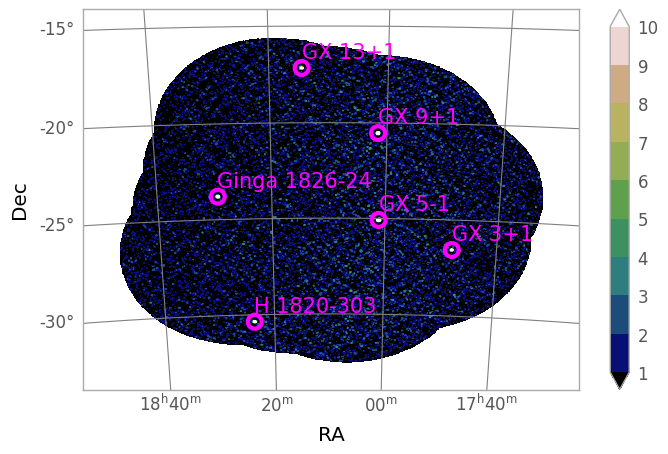
\includegraphics[width = 13cm]{report/Figures/methods/2204/oda_2204.png}
        \caption{Mosaic made with the precedent images using the \texttt{ODA} plot tools for the 22.04.2022 data.}
        \label{22_mosaic}
        \end{figure}
    
    \textbf{24.04.2022 data}
    
    The same process is done with the April 24 data which consists of four scws. \textbf{Fig.} \ref{24_map_single} shows the flux map for the first scw of the list shown on \textbf{Tab.} \ref{journal}. All the other flux maps are presented in the \textbf{Annex A}. \textbf{Fig.} \ref{24_mosaic} shows a mosaic done using all valid scws from the list with the \texttt{ODA}.

        \begin{figure}[H]
        \centering
        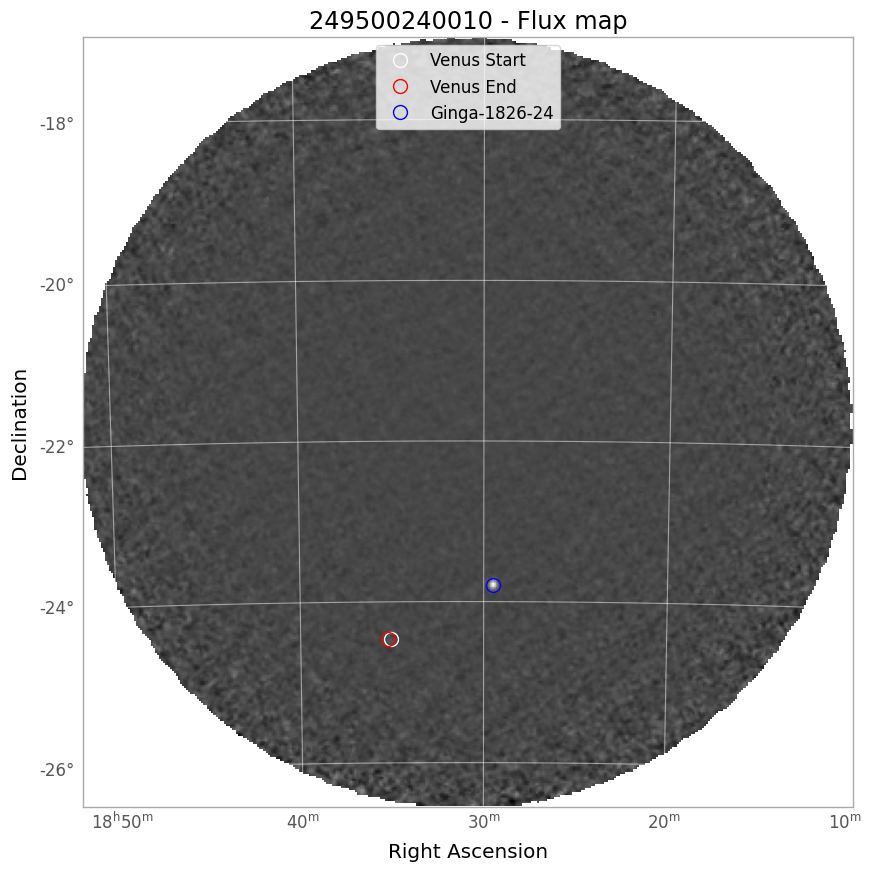
\includegraphics[width = 8cm]{report/Figures/methods/2404/24_map.png}
        \caption{Flux map from the first scw where Venus is present on the 24.04.2022. The start and end positions of Venus are circled in white and red respectively. Another bright source is also plotted to verify the correct localisation approach. Here it is the X-ray binary Ginga 1826-24.}
        \label{24_map_single}
        \end{figure}


        \begin{figure}[H]
        \centering
        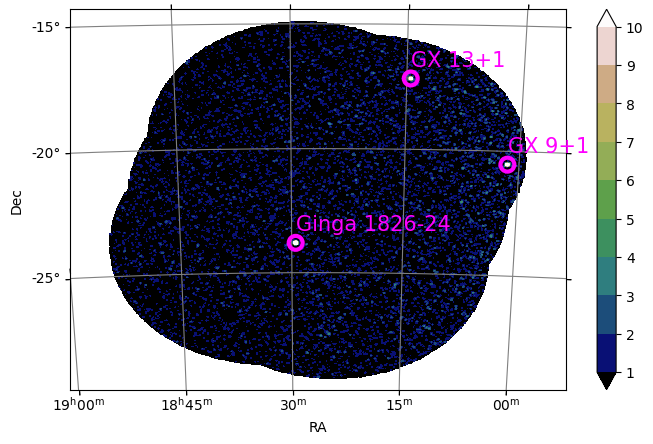
\includegraphics[width = 12cm]{report/Figures/methods/2404/oda_2404.png}
        \caption{Mosaic of the 24.04.2022 data.}
        \label{24_mosaic}
        \end{figure}

    
    \subsection{Models and assumptions}

    Three different models are used to retrieve the fluxes from Venus' position in the data arrays. The first idea is a really simple one: since Venus' apparent size is smaller than a pixel on the image, the idea is to take the value of the pixel Venus is in. This value can vary as Venus travels across the image. The uncertainty on the flux obtained is given by the square root of the value obtained for the same pixel in the variance map. The uncertainty is given at the $3\sigma$-level representing a 99.7\% confidence internal assuming a normal distribution of the possible values.

    The second way of finding the flux emitted at Venus' position is to fit the sum of 2D Gaussian functions on the position of Venus. This function should represent the Point-Spread Function (PSF) of the JEM-X detector. The only free parameter optimised during the fit is the height of the Gaussian. The width is fixed by JEM-X's resolution of 3' meaning that $\sigma_x=\sigma_y=0.82$ pixel. The center of the Gaussian is given by the position of Venus at the time of measurement.  Since the planet moves in the image, it is a sum of 2D Gaussians that is fitted where the number of summed elements is two for simplicity: one for the start position of Venus in the scw and for the end position. From there, two assumptions can be made concerning the parameters to optimise which are the heights of each summed 2D Gaussian: the flux of Venus can be assumed to be constant in the whole scw or it can also be assumed that the flux has a variability smaller than the scw time frame and then both summed Gaussians' heights are optimised. \cite{Dennerl2002DiscoveryChandra} actually finds that the temporal variability of Venus' flux in the soft X-rays has a temporal variability of minutes like the solar flux. It is therefore interesting to test both ideas.

    The functions fitted are the following:

    \begin{equation}
        f(x,y) = h + h_1e^{-\left(\frac{(x-x_0)^2}{2\cdot \sigma_x^2} + \frac{(y-y_0)^2}{2\cdot \sigma_y^2}\right)} +h_2e^{-\left(\frac{(x-x_0)^2}{2\cdot \sigma_x^2} + \frac{(y-y_0)^2}{2\cdot \sigma_y^2}\right)},
    \end{equation}
    where $h_1 = h_2$ is the constant flux assumption and $h_1\neq h_2$ in the other case. The minimisation of the objective function is done using the \texttt{minimize} function of the \texttt{scipy} library. \textbf{Fig.} \ref{model_psf_const} and \ref{model_psf_notconst} show respectively the constant and non constant flux assumptions models
        \begin{figure}[H]
        \centering
        \begin{subfigure}{.45\textwidth}
            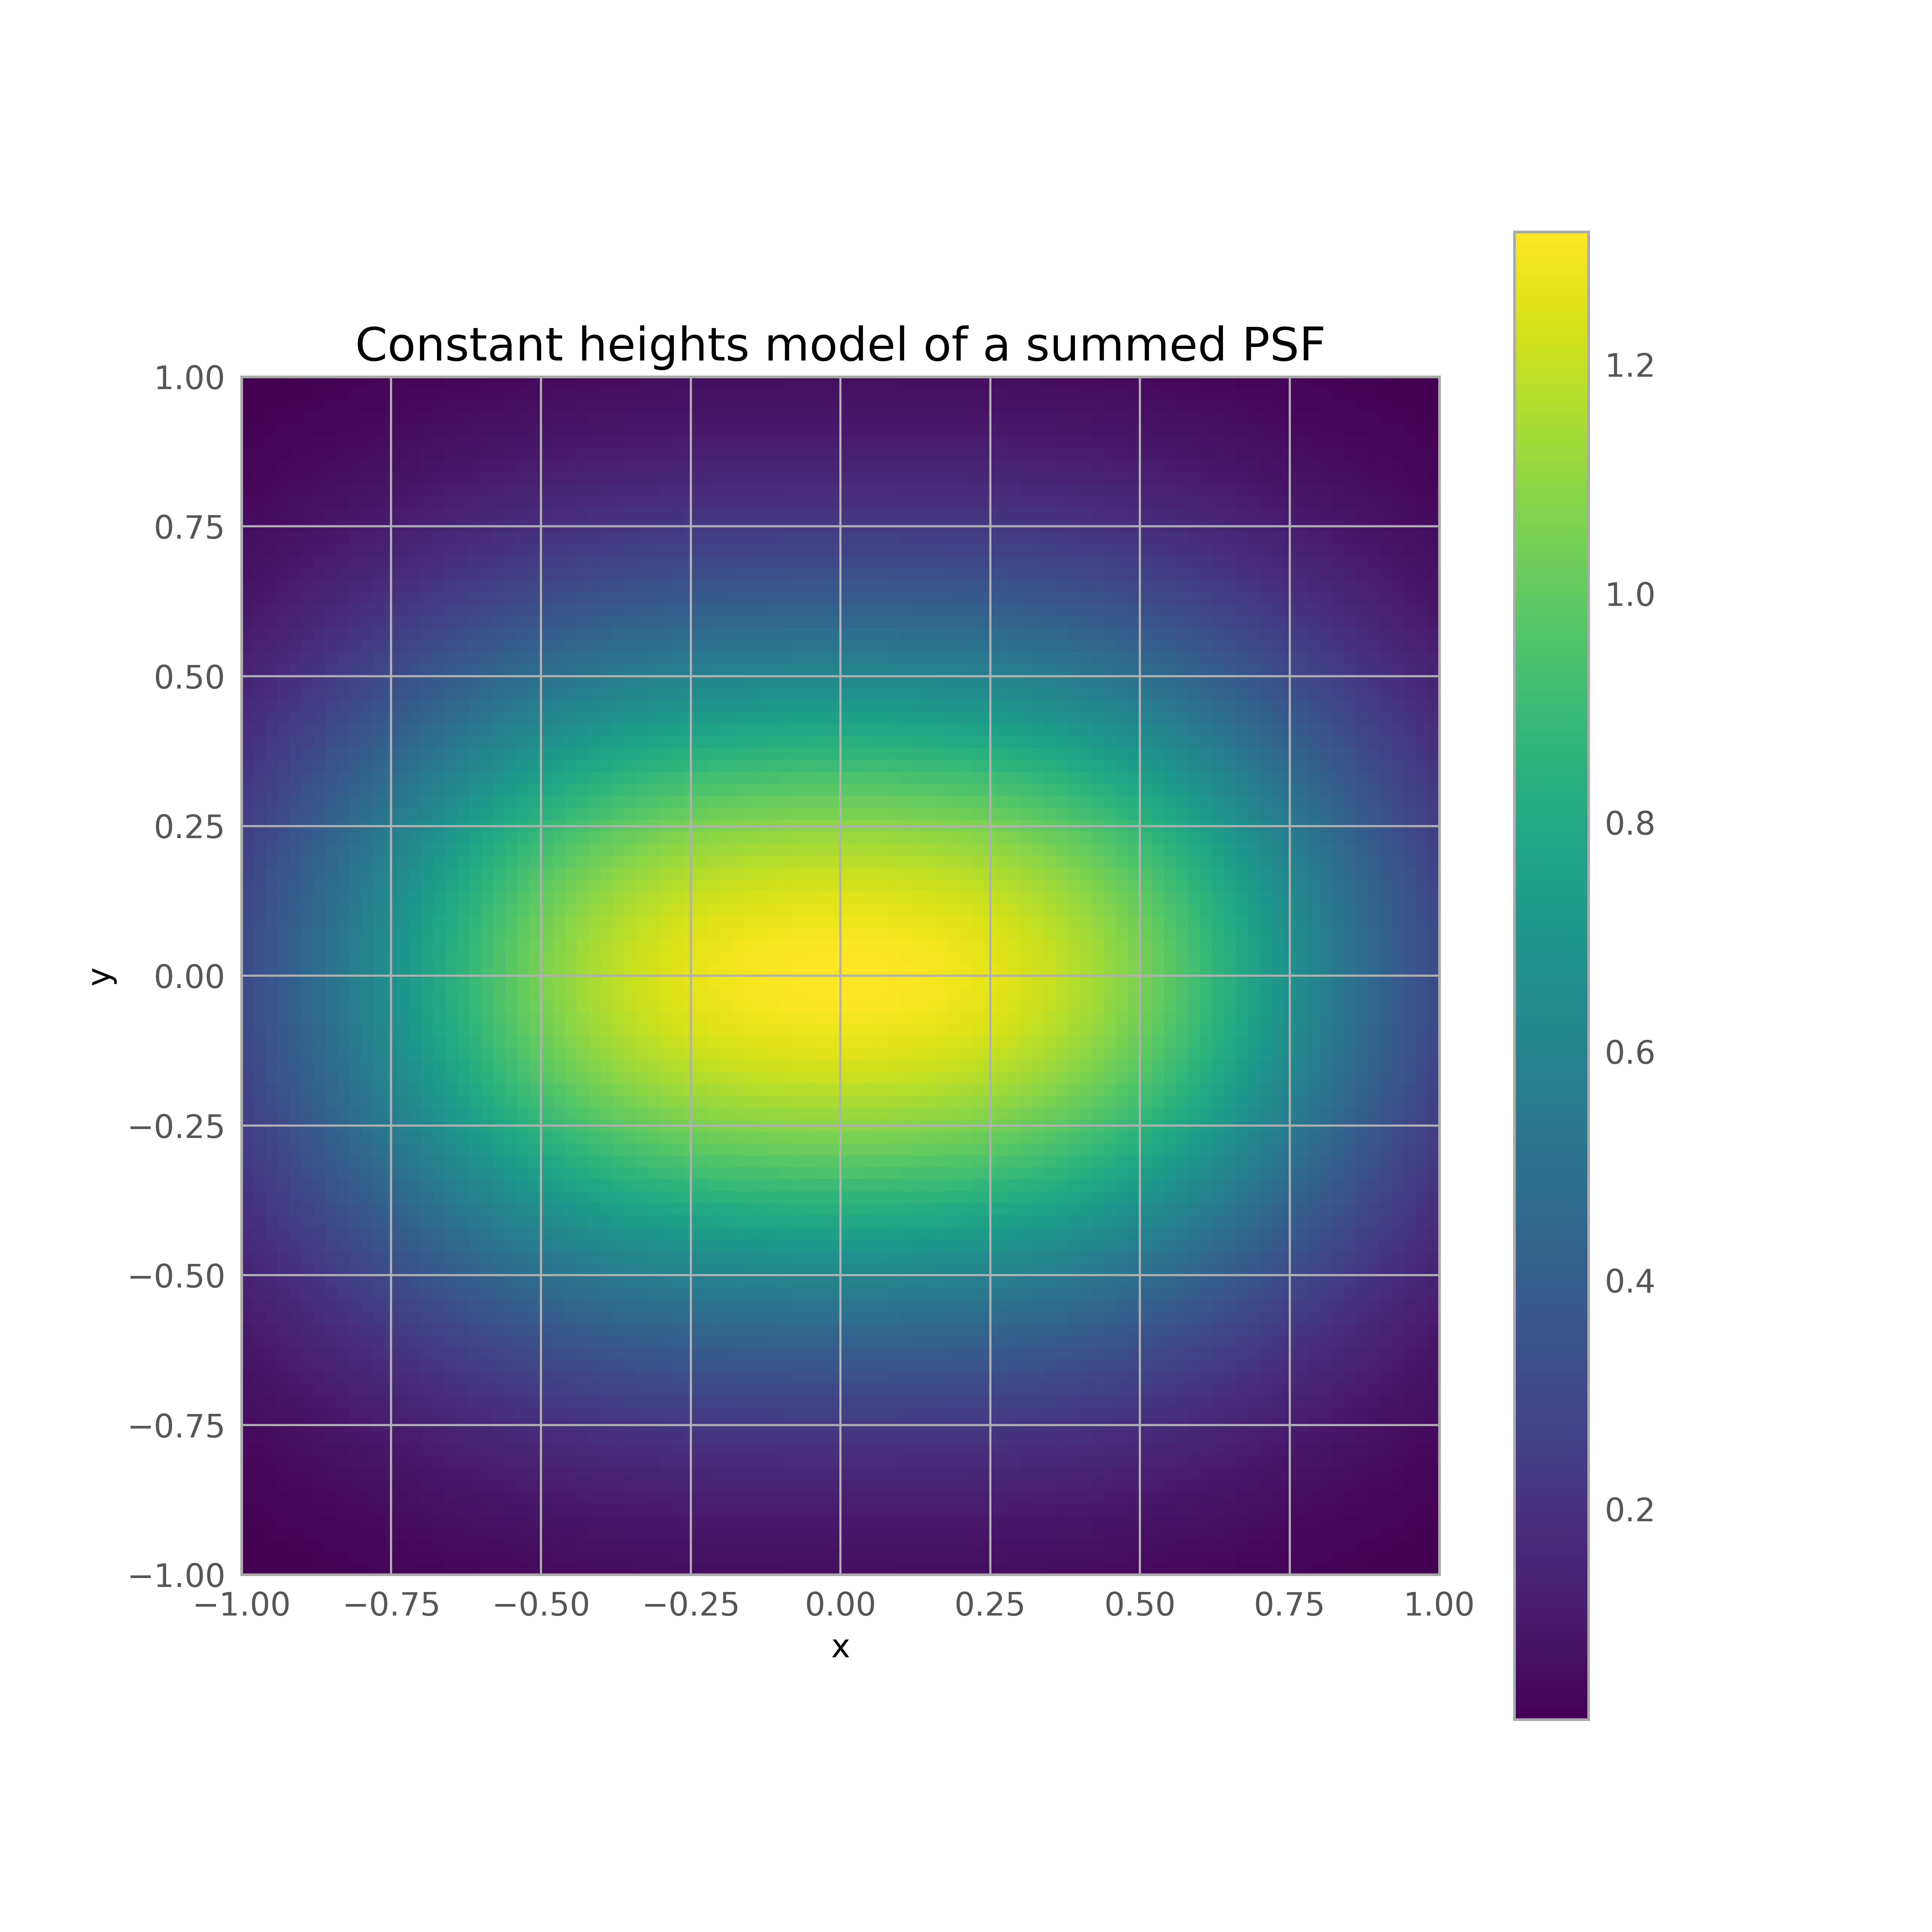
\includegraphics[width=\textwidth]{report/Figures/models/model_psf_const.png}
        \end{subfigure}%
        \hspace{1em}-
        \begin{subfigure}{.45\textwidth}
            \centering
            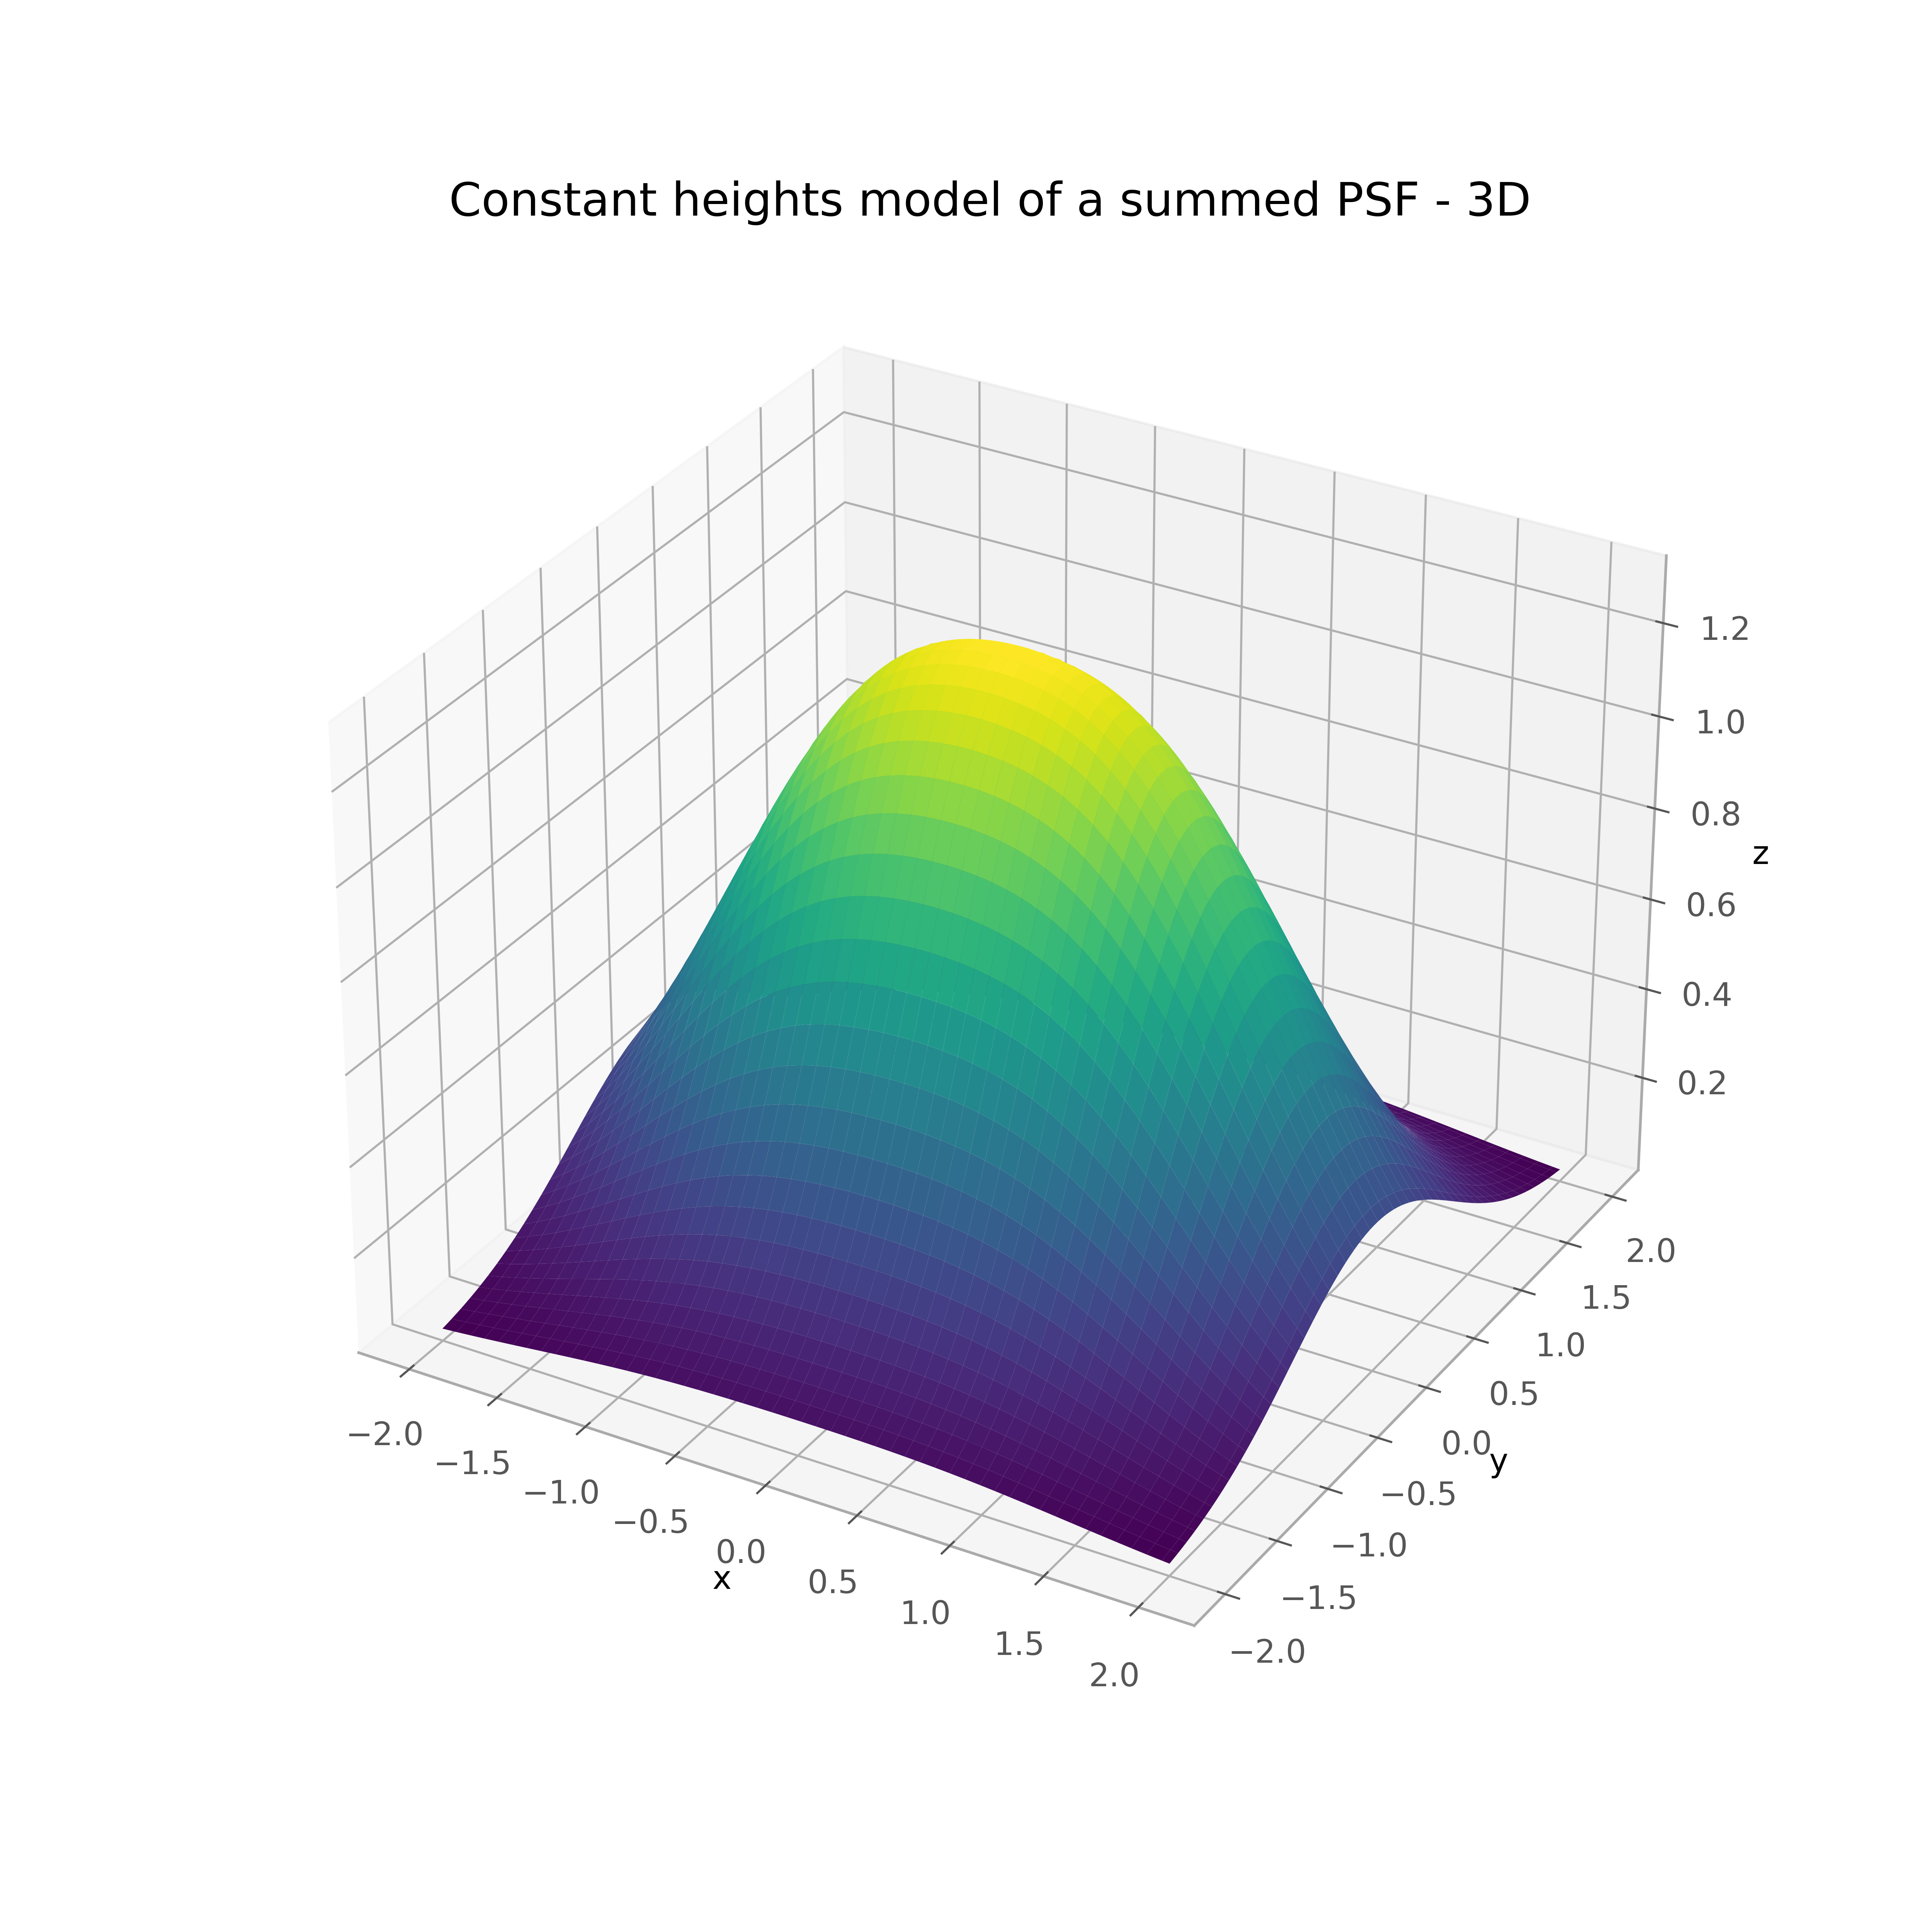
\includegraphics[width=\textwidth]{report/Figures/models/model_psf_const_3d.png}
        \end{subfigure}
        \caption{Constant summed PSFs used as models for Venus' flux.}
        \label{model_psf_const}
        \end{figure}


        %explain here why it's relevant to have a psf not const: because the time variability of venus can be of order of sun(see chandra paper).


        \begin{figure}[H]
        \centering
        \begin{subfigure}{.45\textwidth}
            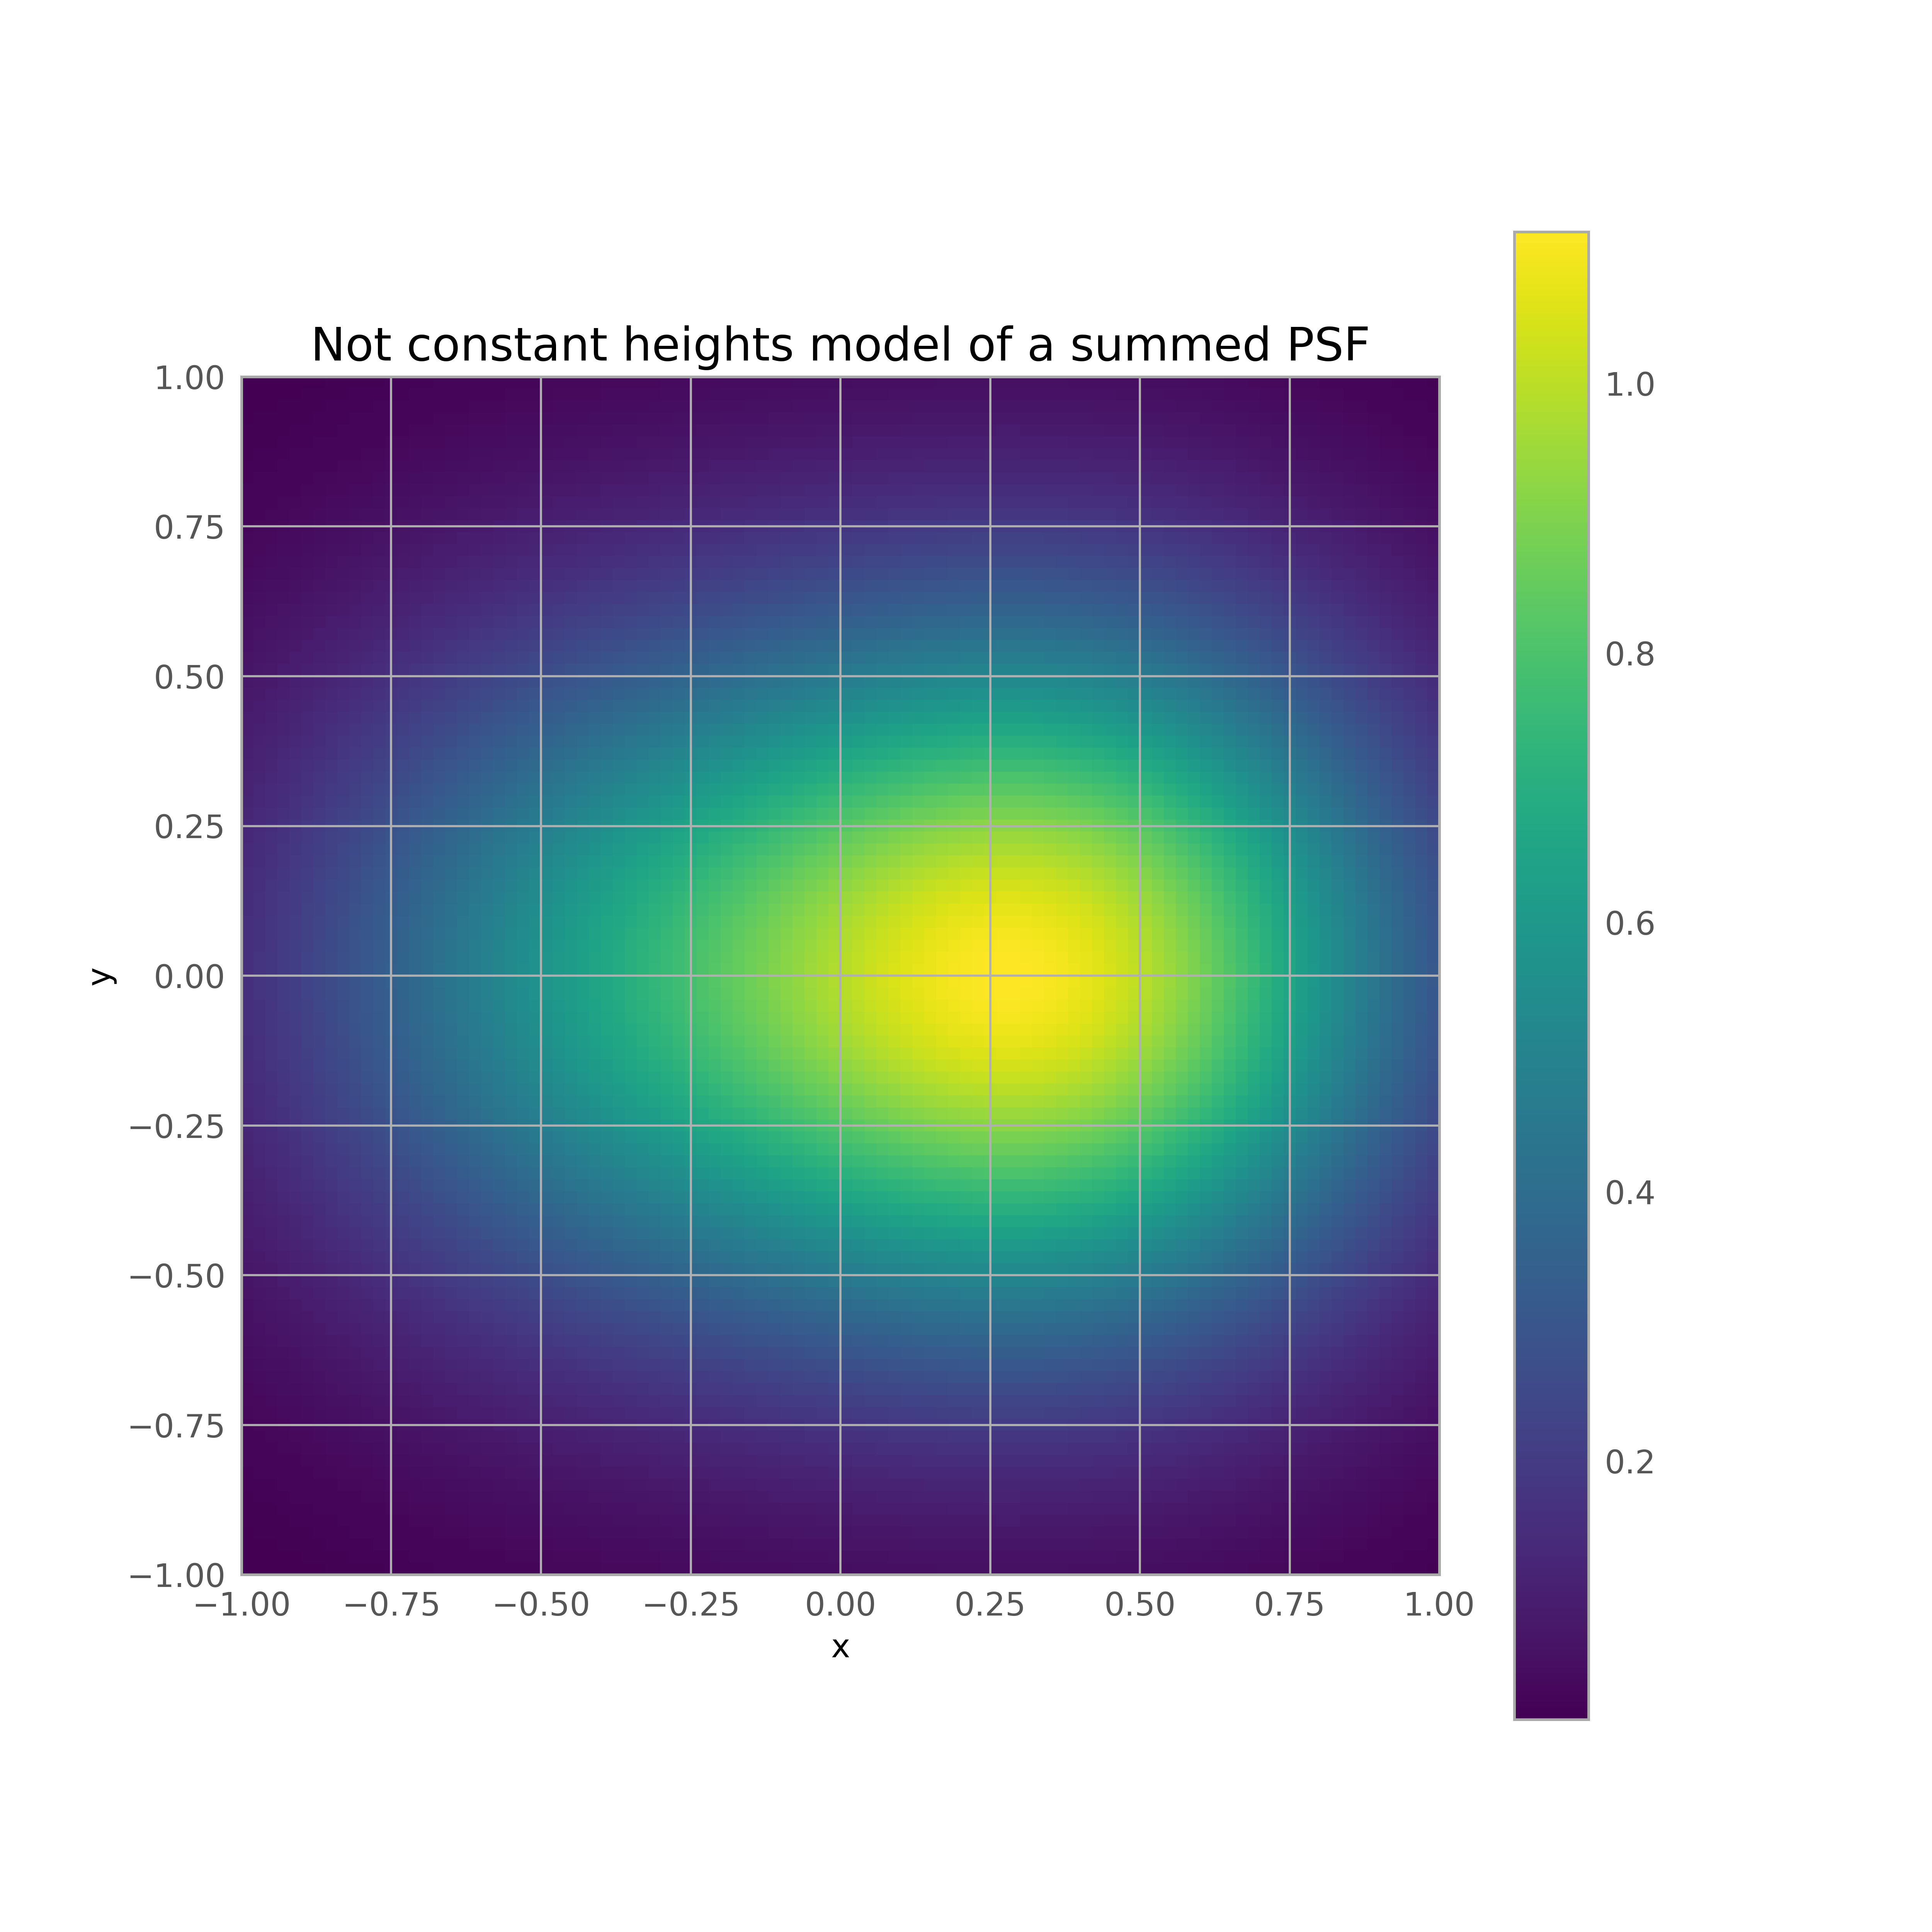
\includegraphics[width=\textwidth]{report/Figures/models/model_psf_notconst.png}
        \end{subfigure}%
        \hspace{1em}-
        \begin{subfigure}{.45\textwidth}
            \centering
            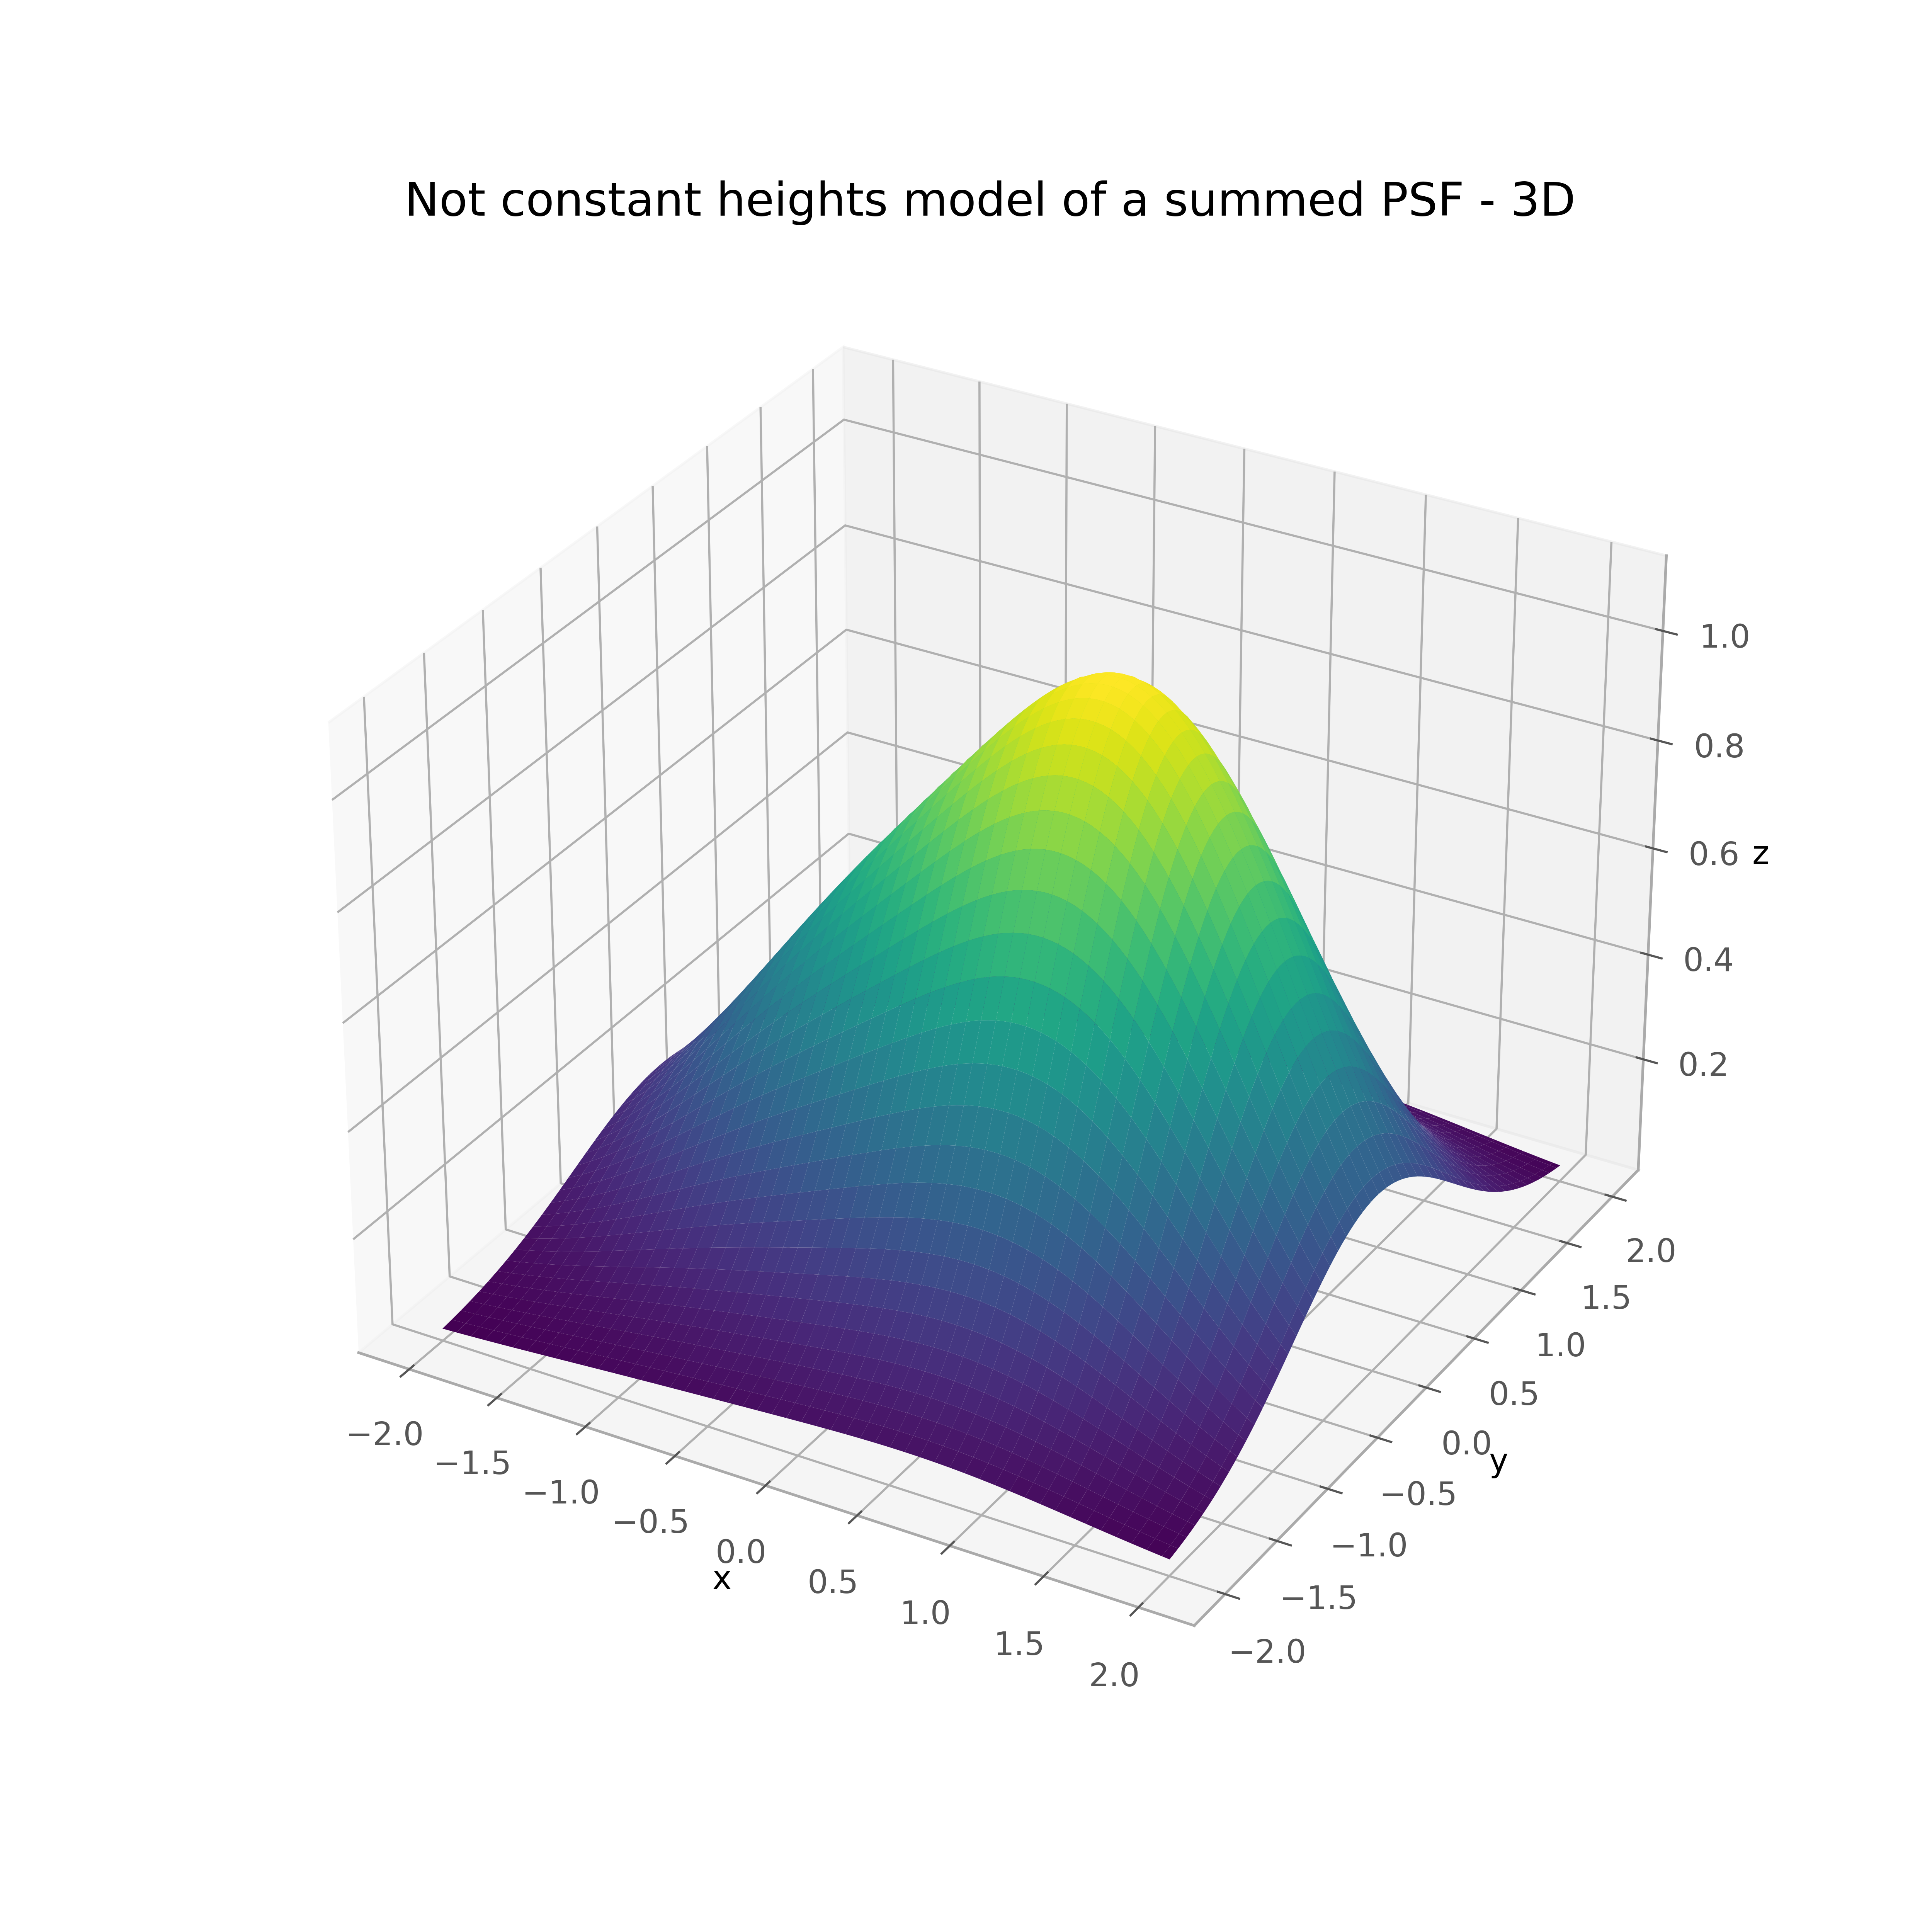
\includegraphics[width=\textwidth]{report/Figures/models/model_psf_notconst_3d.png}
        \end{subfigure}
        \caption{Non constant summed PSFs used as models for Venus' flux.}
        \label{model_psf_notconst}
        \end{figure}

        The uncertainty on the optimised height can be obtained in different ways. One is obviously MC sampling. The simpler way used here is to compute the relative deviations from the best-fitted height when scanning the heights around the optimised value gotten from the minimisation process. The deviations $D$ are computed as follows from the residuals $r_i = $ (data - fitted model) of each pixel $i$ in a cropped square of 20 pixels centered on the start position of Venus:
        \begin{align}
            \chi^2 &= \sum_i r_i^2, \\
            D &= \frac{\chi^2-\chi_{best\, fit}^2}{\chi_{best\, fit}^2} 
        \end{align}
        
        The deviation threshold is set at 2\%. The uncertainty on each point is then obtained by finding the interval when intersecting the $D(height)$ function with an horizontal line representing the 2\% threshold. The deviations for each point of the 22.04 scws are shown on \textbf{Fig.} \ref{threshold}. The same is done for the 24.04 scws.

        \begin{figure}[H]
        \centering
        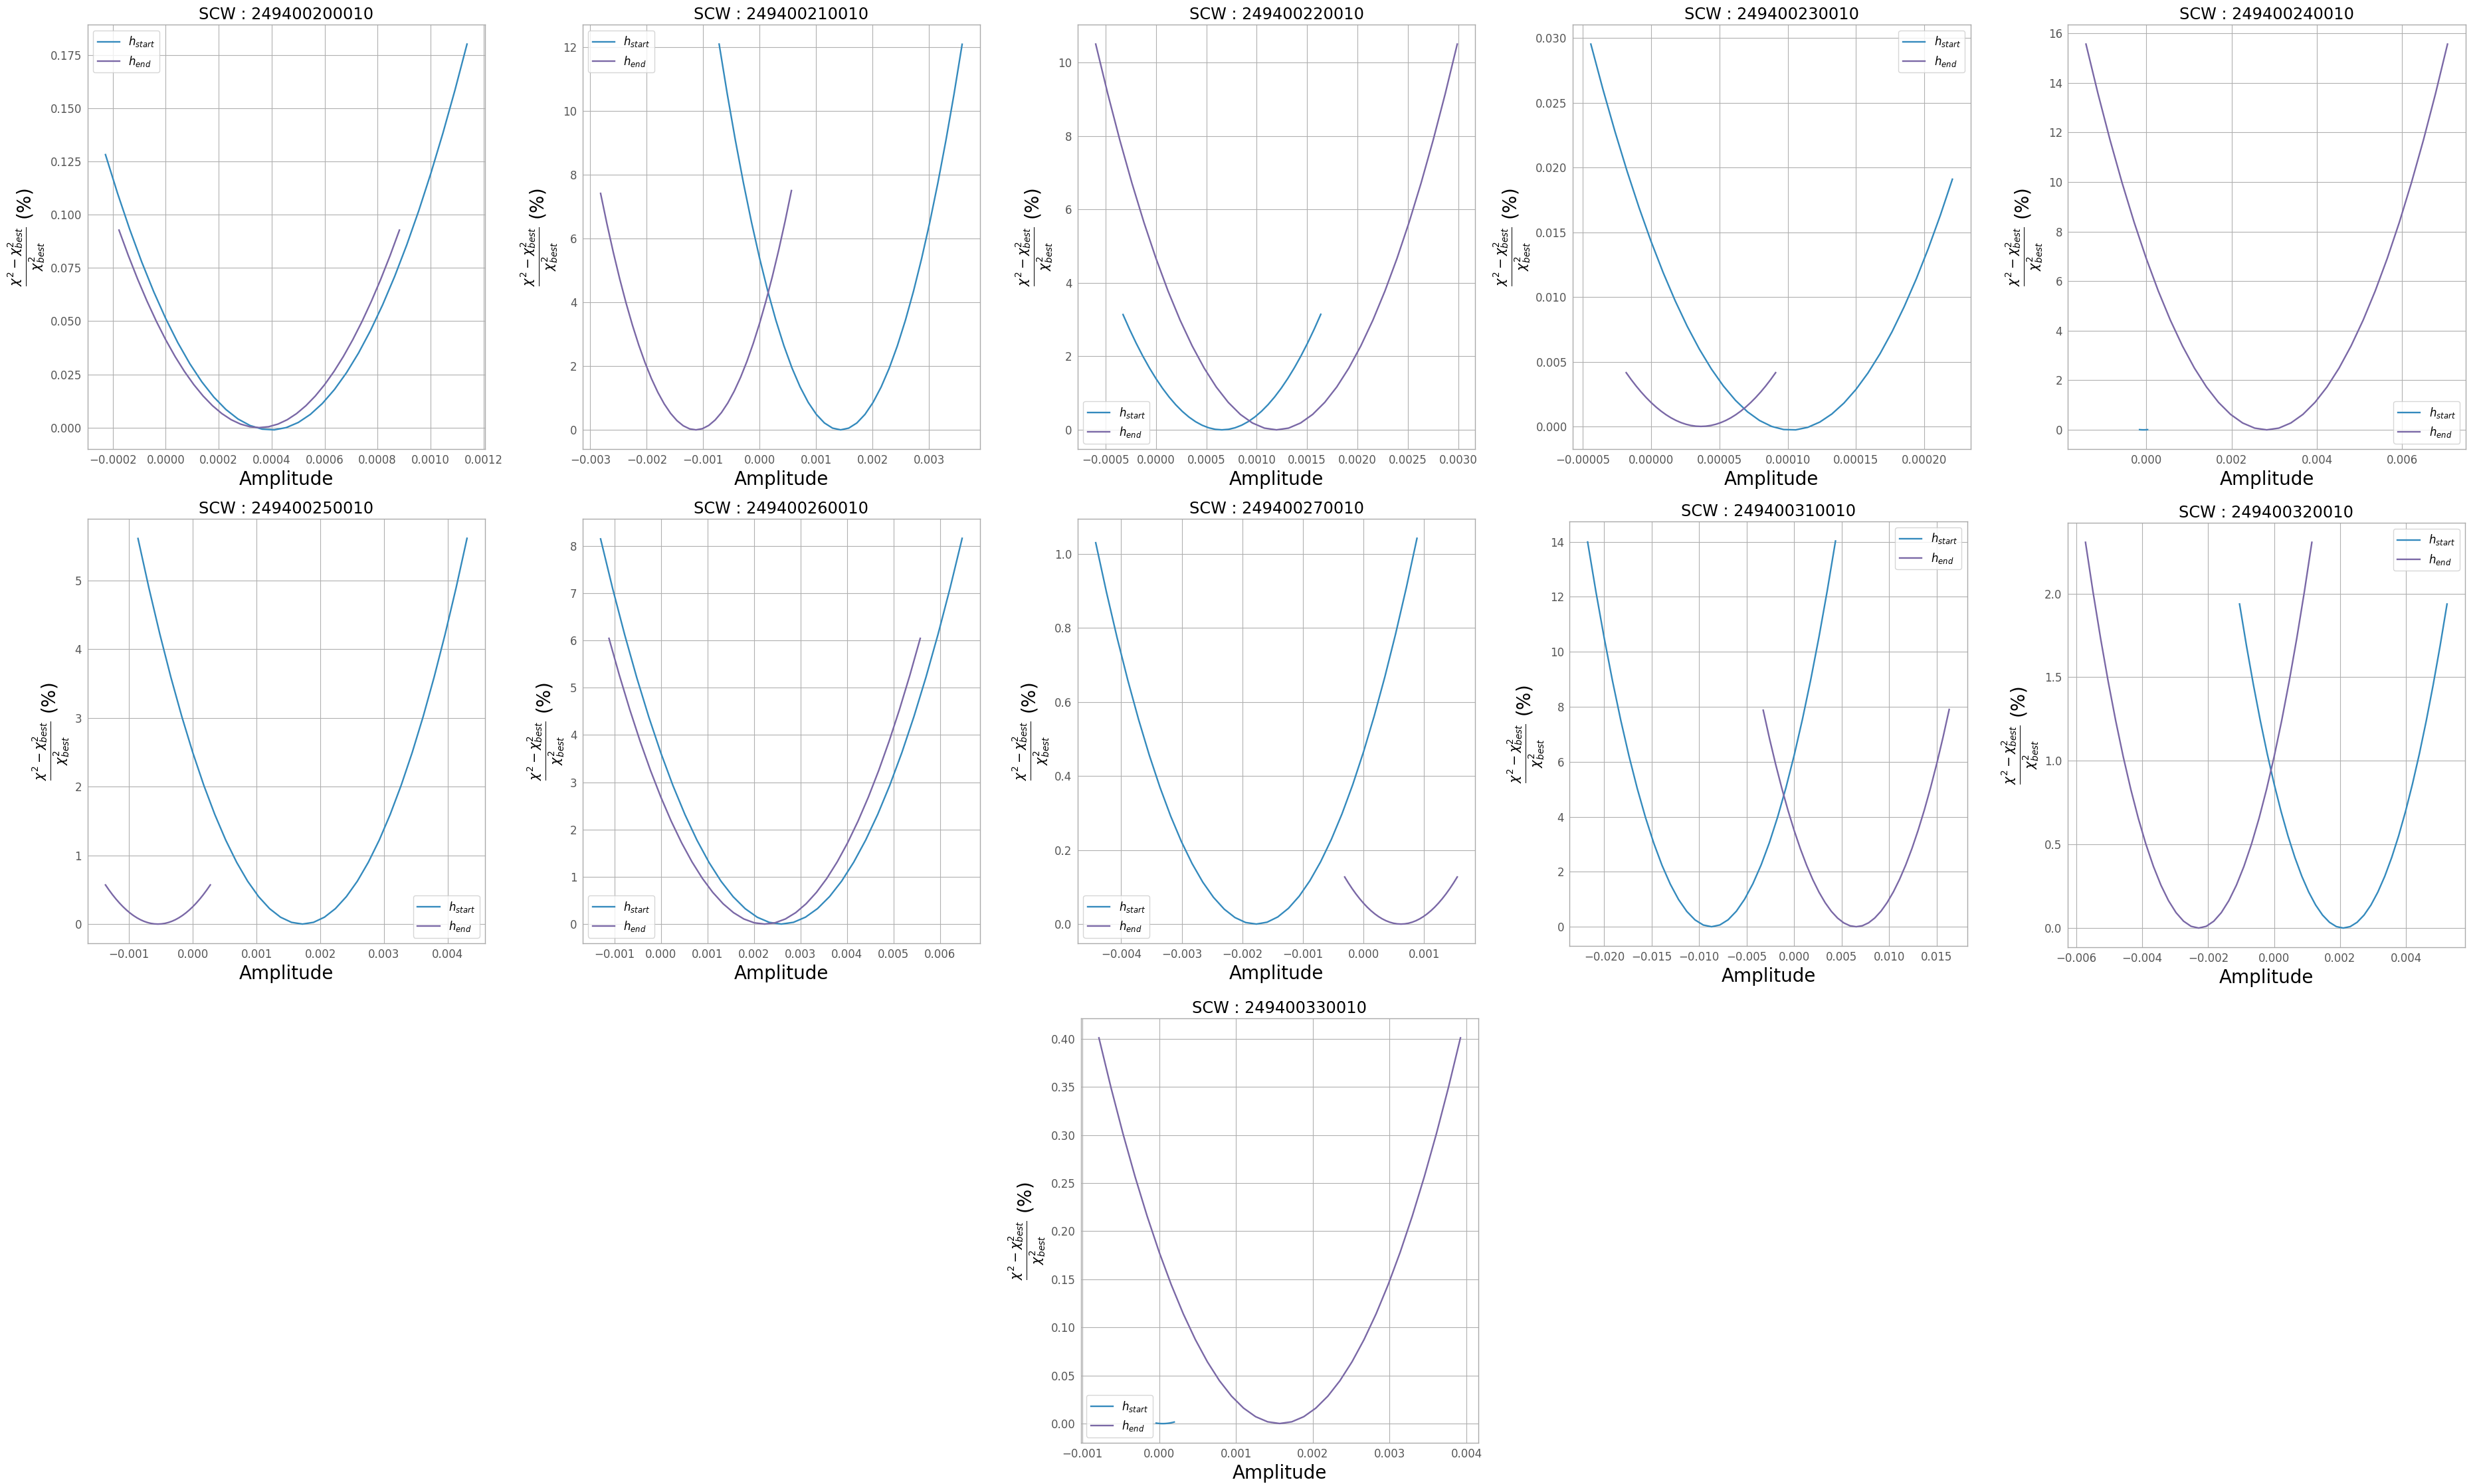
\includegraphics[width = \textwidth]{report/Figures/models/2204/threshold_determination_notconst.png}
        \caption{Normalised deviations from the optimised height for each flux point. The threshold is set at 2\% of the best-fit value.}
        \label{threshold}
        \end{figure}

    
    %--------------------------------------------------
    
    \subsection{Solar events}

    The GOES spacecrafts are a series of geostationary meteorological satellites orbiting the Earth and providing information on space weather too. The GOES-16 satellite, currently in operation, monitors the solar X-ray flux in two different channels: \textit{XRSA} (1-8 \AA) and \textit{XRSB} (0.5-4 \AA). 

    The XRSA channel corresponding to energies ranging from 1.5 kev to 12.4 keV is used here. The solar flux in this channel for every day between the 19.04.2022 and 24.04.2022 is shown on \textbf{Fig.} \ref{goes_tot}.

    The GOES satellites also monitor solar flares and classes them automatically. The CME are mostly monitored by other space telescopes such as SOHO via the LASCO detector. All these events are archived in the \href{https://docs.sunpy.org/en/stable/generated/api/sunpy.net.hek.HEKClient.html}{Heliophysics Knowledge Database} (HEK) accessible through the \texttt{Sunpy} library. The surface coordinates of the events are given in the Helioprojective coordinate system (HPC). In order to find the direction of each event in the solar system, a transformation has to be made to the Heliographic Stonyhurst frame  (HGS). The \texttt{Sunpy} library contains built-in functions enabling these transformations from the ICRF to HGS and HPC to HGS. \textbf{Fig.} \ref{coordinates} illustrates the different coordinate systems in the \texttt{Astropy} and \texttt{Sunpy} packages.

    \begin{figure}[H]
        \centering
        
\includegraphics[width = \textwidth]{report/Figures/methods/GOES_total.png}
        \caption{Solar flux in the XRSA channel(1.5-12.4 keV) of the GOES-16 spacecraft from the 19.04.2022 to the 24.04.2022. The solar flare classes are delimited on the right of each plot.}
        \label{goes_tot}  
    \end{figure}
    
    \begin{figure}[H]
        \centering
        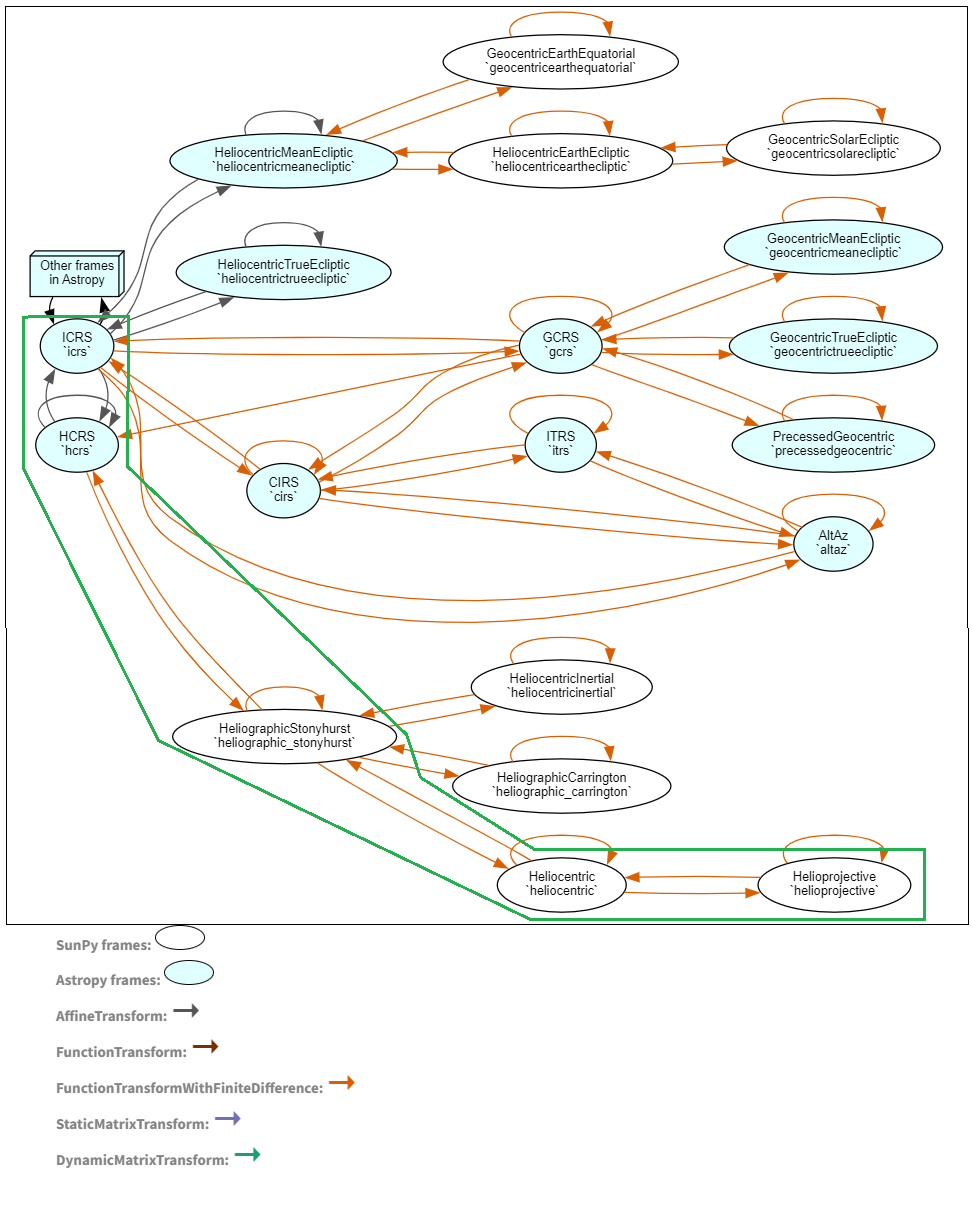
\includegraphics[width = 8cm]{report/Figures/methods/coordinates.png}
        \caption{\texttt{Sunpy} and \texttt{Astropy} coordinate frames transformations. The path used for this study is boxed in green.}
        \label{coordinates}
    \end{figure}

